%This work is licensed under the Creative Commons License Attribution 4.0 International (CC-BY 4.0)
%https://creativecommons.org/licenses/by/4.0/legalcode
% Copy of T02_Graph_B
\documentclass[rgb]{standalone}
\usepackage{tkz-euclide}
\definecolor{myorange}{hsb}{0.0833, 1, 0.8}
\definecolor{mygreen}{hsb}{0.3333, 1, 0.8}
\definecolor{myblue}{hsb}{0.5833, 1, 0.8}
\definecolor{mymagenta}{hsb}{0.8333, 1, 0.8}
\begin{document}
	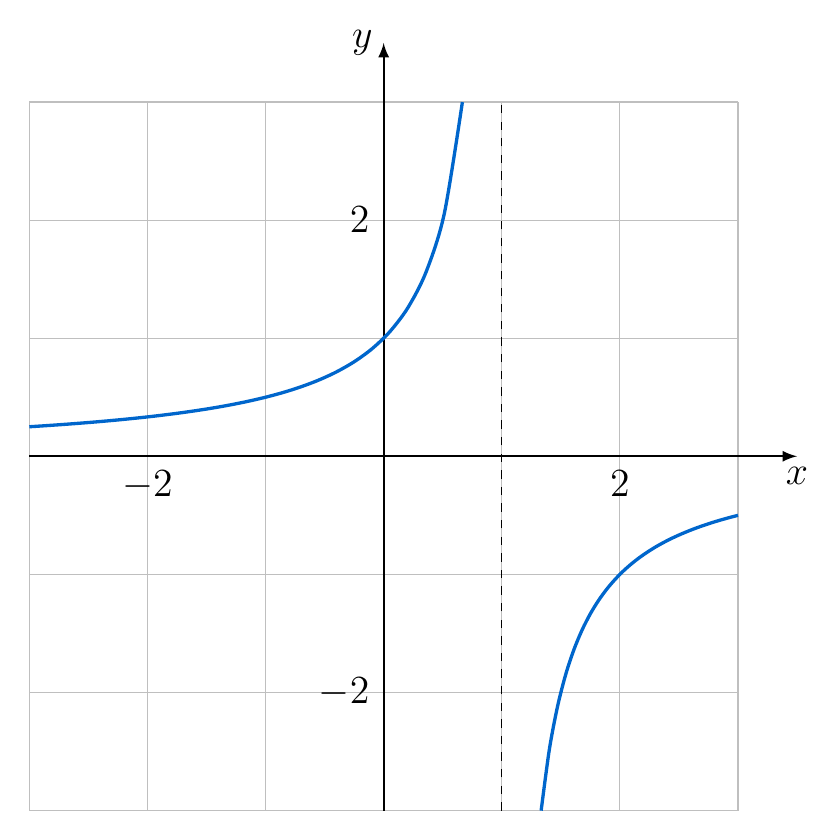
\begin{tikzpicture}[scale=1.5, font=\Large]
		% Coordinate system
		\tkzInit[xmin=-3,xmax=3,ymin=-3,ymax=3]
		\tkzGrid[color=lightgray]
		\tkzDrawX[thick,label=$x$]
		\tkzDrawY[thick,label=$y$]
		% Graph
		\draw[very thick,domain={-3}:{2/3}, smooth, variable=\x, myblue] plot ({\x}, {1/(1-\x)});
		\draw[very thick,domain={4/3}:{3}, smooth, variable=\x, myblue] plot ({\x}, {1/(1-\x)});
		\draw[dashed] (1,-3) -- (1,3);
		% Labels
		\node[below=0.5mm] at (-2,0){$-2$};
		\node[below=0.5mm] at (2,0){$2$};
		\node[left=0.5mm] at (0,-2){$-2$};
		\node[left=0.5mm] at (0,2){$2$};
	\end{tikzpicture}	
\end{document}